\section{Time Evolution}

    \begin{frame}[t]
        \frametitle{Goal of the Calculation}

        \begin{itemize}
            \item Evaluate the time-evolution of the system for various observables \pause
            \begin{itemize}
                \item Uses calculation in the \emph{Interaction Picture} \pause
                \item Introduce operator-less \emph{effective Hamiltonian}
            \end{itemize}
        \end{itemize}

        \vspace{1cm}

        \makebox[\textwidth][c]{
            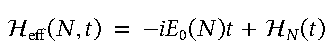
\includegraphics[width=0.165\textwidth,page=1]{main-content/time-evolution/effective-hamiltonian-definition.pdf}
            \includegraphics[width=0.45\textwidth,page=2]{main-content/time-evolution/effective-hamiltonian-definition.pdf}
        }

        % notes 
        \onslide % on all slides of frame
        \note[item] {
            Goal: evaluate the time-evolution for different observables (effectively)
        }
        \note[item] {
            Brute-force calculation is at least NP-hard, definitely exponential and one of the hardest problems to solve computationally generally
        }
        \note[item] {
            Strategy: perform a controlled expansion in the perturbation V and re-express the formulas as a dependency on a operator-free "effective Hamiltonian"
            \begin{itemize}
                \item Can be re-ordered without concern as no operators
                \item For the re-formulation we will use the interaction picture
            \end{itemize}
        }
        \note[item] {
            Particle-type dependency is stored in this formula in the BASE STATES.
            Because in this re-formulation, the Heff is a pure number (no operator) and the initial state is a number (not operator dependent at all).
            But the base-state contains different info for fermions than for bosons, as the operators for hc-bosons commute and so the base-states are uniquely defined. But there are multiple possibilities for teh fermions, because swaps introduce minus signs. (State is not just 0s and 1s, but vacuum that is pre-set with operators and they have an order!!!!!) 
        }
    \end{frame}

    \begin{frame}[t]
        \frametitle{The effective Hamiltonian}

        \makebox[\textwidth][c]{
            \includegraphics[width=0.55\textwidth,page=3]{main-content/time-evolution/effective-hamiltonian-definition.pdf}
        }

        \pause
        \begin{itemize}
            \item Constructed from the contributions of the base energy and the perturbation \pause
            \item Base energy contribution:
        \end{itemize}

        \makebox[\textwidth][c]{
            \includegraphics[width=0.65\textwidth,page=4]{main-content/time-evolution/effective-hamiltonian-definition.pdf}
        }

        % notes 
        \onslide % on all slides of frame
        \note[item] {
            Comprised of two parts:
            \begin{itemize}
                \item Simple, quickly stated term that depends on the base energy 
                \item Complicated one that will be expanded in the perturbation
            \end{itemize}
        }
    \end{frame}

    \begin{frame}[t]
        \frametitle{The effective Hamiltonian}

        \begin{itemize}
            \item To evaluate the time-evolution of the perturbation
        \end{itemize}

        \makebox[\textwidth][c]{
            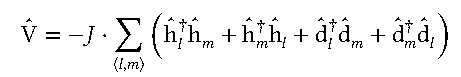
\includegraphics[width=0.50\textwidth,page=1]{main-content/time-evolution/v-in-interaction.pdf}
        }

        \pause
        \begin{itemize}
            \item Solve the equation of motion for the ladder operators
        \end{itemize}
        
        \vspace{-0.1cm}
        \makebox[\textwidth][c]{
            \includegraphics[width=0.50\textwidth,page=2]{main-content/time-evolution/v-in-interaction.pdf}
        }


        % notes 
        \onslide % on all slides of frame
        \note[item] {
            Need: V-Operator in the Interaction picture 
        }
        \note[item] {
            For that: first solve the equations of motion for the ladder operators and the plug in
        }
        \note[item] {
            Solving the equations of motions in the interaction picture requires their number operator being \emph{idempotent}
        }
    \end{frame}

    \begin{frame}[t]
        \frametitle{The effective Hamiltonian}

        \begin{itemize}
            \item Insert and reorder the operators
        \end{itemize}

        \makebox[\textwidth][c]{
            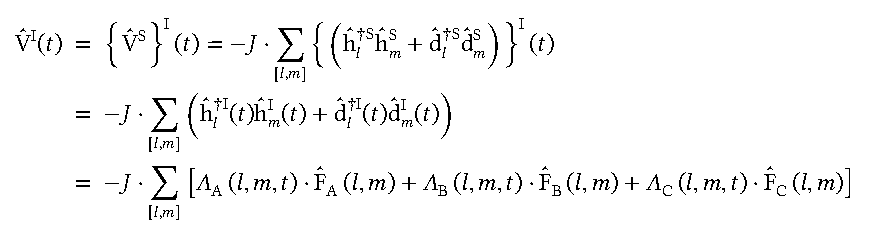
\includegraphics[width=0.80\textwidth,page=1]{main-content/time-evolution/v-in-interaction-solution.pdf} % TODO
        }%
        \vspace{-0.0cm}
        \pause
        \makebox[\textwidth][c]{
            \includegraphics[width=0.80\textwidth,page=2]{main-content/time-evolution/v-in-interaction-solution.pdf}
        }

        % notes 
        \onslide % on all slides of frame
        \note[item] {
            Inserting yields TWO kinds of terms
            \begin{itemize}
                \item time-dependent analytical pre-factors (or their integral as one sees later)
                \item dressed hopping terms, basically only depending on the occupation of the state N
            \end{itemize}
        }
    \end{frame}

    \begin{frame}[t]
        \frametitle{The effective Hamiltonian}

        \begin{itemize}
            \item Evaluate the contribution to the effective Hamiltonian \pause
            \begin{itemize}
                \item Requires previously calculated value of the V-operator in the Interaction Picture \pause
                \item Controllable \emph{cumulant expansion}
            \end{itemize}
        \end{itemize}

        \pause[2]
        \vspace{0.2cm}
        \makebox[\textwidth][c]{
            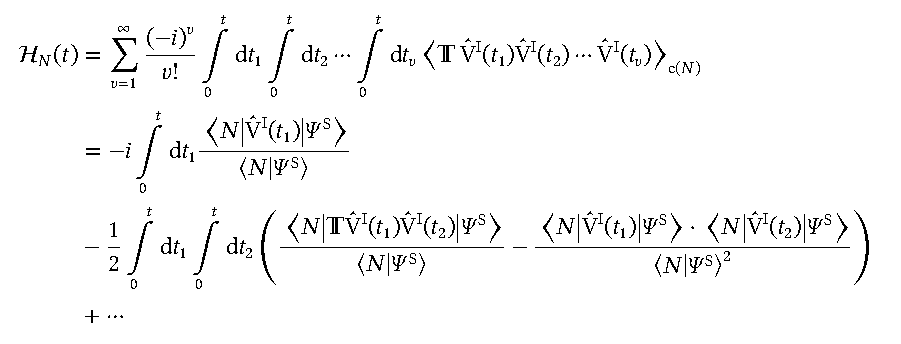
\includegraphics[width=0.80\textwidth,page=1]{main-content/time-evolution/effective-hamiltonian-n.pdf}
        }

        % notes 
        \onslide % on all slides of frame
        \note[item] {
            Generally any expansion possible, but here we expand the \emph{argument of the exponential} - cumulant
        }
        \note[item] {
            first order easily derivable with the info from the previous slide (integrate)
        }
        \note[item] {
            second and higher orders very complicated occupation terms and the pre-factors require quite a lot of edge-cases to integrate with the time-ordering operator
            \begin{itemize}
                \item Hint onto the thesis for this exact derivation
            \end{itemize}
        }
    \end{frame}

    \begin{frame}[t]
        \frametitle{Handling of Observables}

        \begin{itemize}
            \item This allows for general evaluation of expectation values \pause
            \begin{itemize}
                \item Requires a probability for the state
                \item Requires a local observable
            \end{itemize}
        \end{itemize}

        \pause[1]
        \vspace{0.2cm}
        \makebox[\textwidth][c]{
            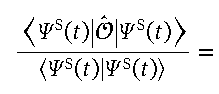
\includegraphics[width=0.28\textwidth,page=1]{main-content/time-evolution/time-evolution-of-observable.pdf}
        }
        \pause[2]
        \makebox[\textwidth][c]{
            \includegraphics[width=0.80\textwidth,page=2]{main-content/time-evolution/time-evolution-of-observable.pdf}
        }

        % notes 
        \onslide % on all slides of frame
        \note[item] {
            Why? General evaluation of an expectation value for an observable.
            \begin{itemize}
                \item Probability for state
                \item Local observable (can be swapped for many different ones)
            \end{itemize}
        }
        \note[item] {
            Does ONLY require difference of effective Hamiltonian for evaluation (notice for later)
        }
    \end{frame}

    \begin{frame}[t]
        \frametitle{Simple Observables}

        \begin{itemize}
            \item Local observable for double occupation measurement \pause
            \begin{itemize}
                \item Observables generally are very sparse matrices
                \item Reduces to pure occupation measurement
            \end{itemize}
        \end{itemize}

        \makebox[\textwidth][c]{
            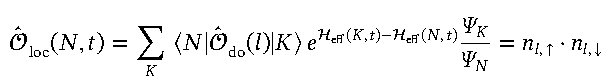
\includegraphics[width=0.7\textwidth,page=1]{main-content/time-evolution/local-observables-simple-ops.pdf}
        }

        \pause
        \begin{itemize}
            \item Local observable for particle current measurement \pause
            \begin{itemize}
                \item Requires evaluation of the difference of two effective Hamiltonians
            \end{itemize}
        \end{itemize}

        \makebox[\textwidth][c]{            
            \includegraphics[width=0.8\textwidth,page=2]{main-content/time-evolution/local-observables-simple-ops.pdf}
        }

        % notes 
        \onslide % on all slides of frame
        \note[item] {
            Complex valued observable, make sure this cancels in the case of approximations
        }
        \note[item] {
            \emph{SHOULD MENTION:} Energy and variance (most expensive ones, are assumed to keep constant, can be used to gauge the quality of the expansion)
        }
    \end{frame}

    \begin{frame}[t]
        \frametitle{Access to Density-Matrics}

        \begin{itemize}
            \item Non-classical (\emph{quantum}) measurements depend on the (reduced) density matrix \pause
                \begin{itemize}
                    \item Access to \emph{purity}, \emph{concurrence} and other entanglement measures/monotones\pause
                \end{itemize}
            \item Direct calculation not possible
        \end{itemize}

        \vspace{-0.2cm}
        \makebox[\textwidth][c]{
            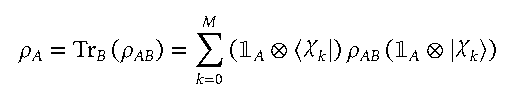
\includegraphics[width=0.65\textwidth,page=1]{main-content/time-evolution/reduced-density-matrix.pdf}
        }

        \vspace{-0.2cm}
        \pause
        \begin{itemize}
            \item Use Pauli matrices to expand the complex 4x4 matrix
        \end{itemize}

        \makebox[\textwidth][c]{
            \includegraphics[width=0.65\textwidth,page=2]{main-content/time-evolution/reduced-density-matrix.pdf}
        }

        % notes 
        \onslide % on all slides of frame
        \note[item] {
            Quite interesting, because of this extra mentioned the Pauli operators
        }
        \note[item] {
            No access to the full density matrix, can not trace out, because too many states to trace out
        }
        \note[item] {
            BUT: as the complex 4x4 matrix can be written in the base of the kronecker product of two pauli matrices, can be expressed (because the pauli operators can be translated into hard-core bosonic ones again and for these we have the general fromula for expectation values)
        }
    \end{frame}

    \begin{frame}[t]
        \frametitle{Access to Density-Matrics}

        \makebox[\textwidth][c]{
            \includegraphics[width=0.75\textwidth,page=3]{main-content/time-evolution/reduced-density-matrix.pdf}
        }

        % notes 
        \onslide % on all slides of frame
        \note[item] {
            Sixteen terms (with missing cases trivially derived from the ones that are given)
        }
        \note[item] {
            Again all depend on the difference of effective hamiltonians between two states ith local modifications
        }
    \end{frame}